% !TeX spellcheck = sl_SI
\documentclass[mat1]{fmfdelo}
% \documentclass[fin1]{fmfdelo}
% \documentclass[isrm1]{fmfdelo}
% \documentclass[mat2]{fmfdelo}
% \documentclass[fin2]{fmfdelo}
% \documentclass[isrm2]{fmfdelo}

% naslednje ukaze ustrezno napolnite
\avtor{Tadej Petrič}
\naslov{ZX-račun}
\title{ZX-calculus}

% navedite ime mentorja s polnim nazivom: doc.~dr.~Ime Priimek,
% izr.~prof.~dr.~Ime Priimek, prof.~dr.~Ime Priimek
% uporabite le tisti ukaz/ukaze, ki je/so za vas ustrezni
\mentor{doc.~dr.~Matija Pretnar}
%\mentorica{izr.~prof.~dr.~Ime Priimek}
%\somentor{doc.~dr.~Ime Priimek}
%\somentorica{doc.~dr.~Ime Priimek}
% \mentorja{}{}
% \mentorici{}{}

\letnica{2021} % leto diplome

%  V povzetku na kratko opišite vsebinske rezultate dela. Sem ne sodi razlaga organizacije dela --
%  v katerem poglavju/razdelku je kaj, pač pa le opis vsebine.
\povzetek{ZX-račun je nov pristop k formalizaciji kvantnega računalništva. Kvantna vezja in procese predstavimo kot barvne grafe z dodatnimi pravili za poenostavljanje, kar omogoči opis vsakega kvantnega vezja. Ogledamo si tudi različne delce ZX računa, ki omogočijo predstavitev različnih modelov kvantnega računalništva. Graf lahko pretvorimo tudi v matriko. Prikažemo tudi nekaj uporab, na primer kvantna teleportacija in kvantno iskanje.}

%  Prevod slovenskega povzetka v angleščino.
\abstract{ZX-calculus is a new approach to the formalization of quantum computing. Quantum circuits are represented with coloured graphs with added simplification rules. Using ZX-calculus, we can describe any quantum circuit. We also explore several fragments of ZX calculus and their use in describing different computational models. The graphs can also be converted to matrices. We also show a few applications, such as the quantum search algorithm and quantum teleportation.}

% navedite vsaj eno klasifikacijsko oznako --
% dostopne so na www.ams.org/mathscinet/msc/msc2010.html
\klasifikacija{81P68}
\kljucnebesede{Kvantno računalništvo, ZX-račun, graf, kategorična kvantna mehanika} % navedite nekaj ključnih pojmov, ki nastopajo v delu
\keywords{Quantum computing, ZX-calculus, graph, categorical quantum mechanics} % angleški prevod ključnih besed

\zapisiMetaPodatke  % poskrbi za metapodatke in veljaven PDF/A-1b standard

% aktivirajte pakete, ki jih potrebujete
\usepackage{tikz}
\usepackage{physics}
\usepackage{mathtools}
\usepackage{csquotes}
\usepackage{biblatex}
\usepackage{tikz}
\usepackage{quantikz}
\usepackage{amsmath}
\usepackage{graphicx}
\addbibresource{sources.bib}

% za številske množice uporabite naslednje simbole
\newcommand{\R}{\mathbb R}
\newcommand{\N}{\mathbb N}
\newcommand{\Z}{\mathbb Z}
\newcommand{\C}{\mathbb C}
\newcommand{\Q}{\mathbb Q}
\newcommand{\Hb}{\mathbb H}

% matematične operatorje deklarirajte kot take, da jih bo Latex pravilno stavil
% \DeclareMathOperator{\conv}{conv}
% na razpolago so naslednja matematična okolja, ki jih kličemo s parom
% \begin{imeokolja}[morebitni komentar v oklepaju] ... \end{imeokolja}
%
% definicija, opomba, primer, zgled, lema, trditev, izrek, posledica, dokaz
%
\definecolor{zx_red}{RGB}{232, 165, 165}
\definecolor{zx_green}{RGB}{216, 248, 216}
\definecolor{had_yellow}{RGB}{221, 218, 28}

\tikzstyle{gn}=[circle,rounded corners=0.8em,fill=zx_green,draw=black,
  line width=0.8 pt,inner sep=3pt,minimum width=1.5em,minimum height=1.5em]
\tikzstyle{rn}=[circle,rounded corners=0.8em,fill=zx_red,draw=black,
  line width=0.8 pt,inner sep=3pt,minimum width=1.5em,minimum height=1.5em]
\tikzstyle{had}=[rectangle,fill=had_yellow,draw=black,
  line width=0.8 pt,inner sep=3pt,minimum width=1.5em,minimum height=1.5em]
% vstavite svoje definicije ...
%  \newcommand{}{}
\newcommand{\defeq}{\vcentcolon=}
\newcommand{\sep}{\ensuremath{.\,}}
\newcommand{\exv}{\langle}
\begin{document}

\section{Uvod}
Koncept kvantnega računalništva se je začel leta 1981, ko je Richard Feynman predlagal, kako bi lahko simulirali določene fizikalne procese z uporabo nekaterih lastnosti kvantne mehanike\cite{feynmann}. Klasični algoritmi imajo namreč težavo, da je časovna zahtevnost simulacije eksponentna glede na njeno velikost. Ker pa je narava teh simulacij pogosto probabilistična lahko uporabimo prednosti kvantne mehanike, ki je tudi sama probabilistična, da jih simuliramo bolj učinkovito, na primer z linearno kompleksnostjo. Na začetku so bili najbolj zanimivi procesi, kjer je potrebno upoštevati kvantno mehaniko -- Feynman je namreč predlagal, da so vsi kvantni sistemi na nek način ekvivalentni. Potem je simulacija preprosta, saj le izvajamo iste korake v kvantnem računalniku, kot se bi izvajali v dejanskem ekspirimentu, za rezultat pa pogledamo končno stanje računalnika.

Izkazalo pa se je, da imajo kvantni računalniki mnogo uporabe tudi izven fizikalnih simulacij: Shorov algoritem sprejme število, in vrne njegove prafaktorje. Ta problem je klasično zelo težek, ne vemo še, ali obstaja učinkovita rešitev, kvantno pa poznamo rešitev, ki deluje hitreje kot eksponentno. Podobno obstaja mnogo drugih težkih problemov za katere imamo hitro kvantno rešitev, na primer iskanje inverzne funkcije, Fourierjeva transformacija, iskanje diskretnega logaritma\ldots

Pomembno vprašanje je kako formalizirati kvantne računalnike in kako jih programirati. John Von Neumann je formaliziral kvantno mehaniko z uporabo Hilbertih prostorov, ta pristop je najbolj pogosto uporabljen še danes\cite{neumann}. Izkaže pa se, da velik del teorije postane bolj naraven, če uporabimo drugačen pristop. To je kmalu predlagal že Neumann z kvantno logiko, vendar se pristop takrat še ni uveljavil, kar je močno obžaloval. Iz kvantne logike se je razvil moderni pristop, kategorična kvantna mehanika. Tukaj lahko mnoge zakone opišemo le z diagrami, kar naredi mnogo dejstev bolj naravnih, ne izgubimo pa nič natančnosti. Iz kategorične kvantne mehanike se je razvil ZX-račun, ki ga uporabljamo za opis kvantnih vrat in vezij z uporabo diagramov. Znotraj samega ZX-računa pa bo marsikaj bolj enostavno, na primer iskanje algoritmov, iskanje novih fizikalnih zakonov in poenostavljanje vezij.

\section{Klasično računalništvo}
Za opis kvantnega računalništva je koristno najprej poznati delovanje klasičnih računalnikov. 
\subsection{Biti in vrata}
Klasični računalniki so zgrajeni na osnovi Boolove algebre. Osnovni objekti so biti, imajo lahko vrednosti \(0\) in \(1\), ustrezajo pa logični neresnici in logični resnici. Namesto \(1\) bomo uporabljali \(\ket{1}\), namesto \(0\) pa pišemo \(\ket{0}\), saj nam to olajša prehod na kvantne računalnike, prav tako pa jih težje zamenjamo z naravnima številoma \(0\) in \(1\). Naredimo množico bitov \(B = \{\ket0, \ket1\}\).

Bite lahko združimo v skupine. Skupina bitov je element kartezičnega produkta množice bitov. Kot primer, skupina treh bitov je \(B^3\), primer elementa te skupine pa je \((\ket0, \ket1, \ket0)\). Uvedemo preprostejši zapis za skupine: 
\begin{align*}
    \ket{a} \defeq& (\ket a)\\
    \ket{ab} \defeq& (\ket{a},\ket b)\\
    \ket{abc} \defeq& (\ket a, \ket b, \ket c)\\
    &\vdots
\end{align*}


\subsection{Primeri}
\subsection{Implementacija}
\subsection{Klasična komunikacija}
\section{Kvantna mehanika}
Klasični pristop do kvantne mehanike uporablja Hilbertove prostore\cite[stran 12]{mathforqm}.

\begin{definicija} \(\Hb\) je Hilbertov prostor če je vektorski prostor s skalarnim produktom
    \begin{align*}
        \braket{\cdot}{\cdot} :& \Hb \times \Hb \to \C\\
        & (\psi, \varphi) \mapsto \braket{\varphi}{\psi},
    \end{align*}
    za katerega za vse \(\phi, \varphi, \varphi_1, \varphi_2 \in \Hb\) velja
    \begin{align*}
        \braket{\psi}{\varphi} &= \overline{\braket{\varphi}{\psi}},\\
        \braket\psi &\geq 0,\\
        \braket\psi = 0 &\iff \psi = 0,\\
        \forall a,b\in\C\sep \braket{\psi}{a\varphi_1 + b\varphi_2} &=a\braket{\psi}{\varphi_1} + b\braket{\psi}{\varphi_2}.
    \end{align*}
    Ta skalarni produkt pa inducira normo
    \begin{align*}
        \norm*{\cdot} : \Hb &\to \R\\
        \psi &\mapsto \sqrt{\braket\psi},
    \end{align*}
    v katerem je \(\Hb\) poln.
\end{definicija}

Linearne preslikave \(\Hb\to\Hb\) so operatorji. Če je \(\forall \psi,\phi\in\Hb\sep\braket{A^*\psi}{\varphi} = \braket{\psi}{A\varphi}\) je \(A^*\) adjungirani operator operatorja \(A\). Operator \(U\) je unitaren če \(\forall \psi,\varphi\in\Hb\sep \braket{U\psi}{U\varphi} = \braket{\psi}{\varphi}\).

Vektorje bomo pisali v Diracovem zapisu. Elementi \(\Hb\) so tako \(\ket{\psi}\in\Hb\), temu rečemo ket. Znotraj skalarnih produktov ketov ponavadi ne pišemo, tako dobimo \(\braket{\ket\psi}{\ket\varphi} = \braket{\psi}{\varphi}\). Elementi dualnega prostora pa so braji:
\begin{align*}
    \bra{\psi} \defeq \left(\varphi \mapsto \braket{\psi}{\varphi} \right).
\end{align*}
Tukaj opazimo, da velja \(\bra{\psi}\, \ket{\varphi} = \braket{\psi}{\varphi}\).

Pomembni so še lastni vektorji in projekcije: \(\ket{\psi}\) je lastni vektor za \(A\) z lastno vrednostjo \(\lambda\), če \(A\ket\psi = \lambda \ket\psi\); \(P\) je projekcija, če \(P^2 = P\). Če je poleg tega še \(P^* = P\) je projekcija ortogonalna.

Za sestavljanje novih Hilbertovih prostorov iz starih nam bo služil tenzorski produkt. Ta nam bo omogočil, da združimo opis dveh kvantnih delcev v en sam sistem. Najprej definiramo tenzorski produkt kot preslikava
\begin{align*}
    \ket\varphi \otimes \ket\psi : \Hb_1 \times \Hb_2 &\to \mathbb C\\
    (u,v) &\mapsto \braket{u}{\varphi}_1 \braket{v}{\psi}_2.
\end{align*}
Linearna ogrinjača takih vektorjev sestavi vektorski prostor \(\Hb_1 \otimes \Hb_2\). Tenzorski produkt večih prostorov naredimo induktivno, najprej tenzorski produkt prvih dveh, dobljenega tenzorsko množimo s tretjim in tako naprej. Prav tako za elemente. Za to nam bo prav prišla oznaka
\begin{align*}
    \ket{\varphi}^{\otimes n} = \bigotimes_{j=1}^n \ket\varphi.
\end{align*}
\subsection{Von Neumannova slika}
\subsubsection{Kvantna stanja in opazljivke}
Kvantna stanja so elementi Hilbertovega prostora \(\ket\psi\in\Hb\), za katere velja \(\norm{\ket\psi} = 1\). Opazljivka je merljiva količina kvantnega sistema (na primer hitrost ali pozicija). Predstavimo jo z sebi-adjungiranim operatorjem \(\Hb\). Definiramo oznako
\begin{align*}
    \ev{A}_\psi = \braket{\psi}{A\psi},
\end{align*}
ki jo imenujemo pričakovana vrednost opazljivke \(A\) v stanju \(\ket\psi\).
\subsubsection{Meritve}
V kvantnih sistemih lahko izmerimo opazljivke. Možni rezultati meritev so točno lastne vrednosti operatorja, ki predstavlja opazljivko. Rečemo da je verjetnost \(P_\psi(\lambda)\), da za kvantni sistem, ki je v stanju \(\ket\psi\) dobimo po meritvi opazljivke \(A\) lastno vrednost \(\lambda\) točno 
\begin{align*}
    P_\psi(\lambda) = \norm{P_\lambda \ket\psi}^2,
\end{align*}
kjer je \(P_\lambda\) projekcija na lastni podprostor z lastno vrednostjo \(\lambda\).
\subsubsection{Spin}
Spin je lastnost osnovnih delcov, podobno kot recimo njihova masa. Fizikalno je spin navidezno vrtenje delcev: imajo vrtilno količino ampak se ne vrtijo. Za osnovne delce bi bilo dejansko vrtenje celo nesmiselno, saj so delci točkasti brez volumna ali polmera. Ne glede na to pa spin še vedno lahko spin še vedno izmerimo, prav tako pa ima mnoge posledice na okolje. V kvantnem računalništvu bomo spin izrabljali za predstavitev kubitov. Da lahko vrednost spina spremljamo uporabimo Paulijeve matrike.
\begin{definicija} Paulijeve matrike so \(2\times 2\) unitarne kompleksne matrike:
    \begin{align*}
        X &= \sigma_x \defeq \begin{bmatrix}
            0&1\\
            1&0
        \end{bmatrix},\\
        Y &= \sigma_y \defeq \begin{bmatrix}
            0&-i\\
            i&0
        \end{bmatrix},\\
        Z &= \sigma_z \defeq \begin{bmatrix}
            1&0\\
            0&-1
        \end{bmatrix}.
    \end{align*}
\end{definicija}
Opazljivke spina dobimo, če Paulijeve matrike delimo z \(2\). Te imajo lastne vrednosti \(\pm \frac12\) in jih uporabimo za meritve v naravi. V navadi pa je, da faktorja \(\frac12\) ne pišemo in kot opazljivke uporabimo le \(\sigma_x\) in \(\sigma_z\).
\subsection{Kubiti}
Kubite definiramo kot elemente Hilbertovega prostora \(\mathbb C^2\) dolžine \(1\). Kot njihove opazljivke uporabimo paulijeve matrike. Če gledamo le spin v \(z\) smeri, uporabljamo opazljivko \(\sigma_z\), ki ima lastne vrednosti \(\{+1, -1\}\). Tem lastnim vrednostim ustrezajo lastni vektorji \(\ket0\) in \(\ket1\), ki jih definiramo kot
\begin{align*}
    \ket0 \defeq \begin{bmatrix}
        1\\0
    \end{bmatrix}\\
    \ket1 \defeq \begin{bmatrix}
        0\\1
    \end{bmatrix}
\end{align*}
Opazimo, da to sestavlja bazo vektorskega prostora. Kubit lahko tako napišemo kot linearno kombinacijo \(\ket0\) in \(\ket1\). Tukaj lahko vidimo vzporednico s klasičnim računalništvom: tam so bili biti le \(\ket0\) in \(\ket1\), tukaj pa tudi vse vrednosti vmes! Eksplicitno, poljubni kubit je oblike \(a\ket0+b\ket1\) kjer \(a^2+b^2=1\).

Definiramo si še Bellova stanja
\begin{align*}
    \ket{+} \defeq \frac{1}{\sqrt2} (\ket0+\ket1)\\
    \ket{-} \defeq \frac{1}{\sqrt2} (\ket0-\ket1).
\end{align*}
Ustrezajo lastnim vektorjem opazljivke \(\sigma_x\), ki spremlja spin v \(x\) smeri. Spina \(X\) in \(Z\) sta dualna, kar ima posledico, da ima vsak izrek o \(Z\) spinu analogno trditev o \(X\) spinu, le vse \(\ket+\) zamenjamo s \(\ket0\) in obratno, prav tako pa zamenjamo \(\ket-\) s \(\ket1\).

Podobno kot pri klasičnem računalniku potrebujemo sisteme več bitov, pri kvantnih računalnikih potrebujemo sisteme večih kubitov. Fizično ga pogosto predstavimo kot računalnik z večimi elektroni, en za vsak kubit. Tukaj uporabimo tenzorski produkt. Sistem dveh kubitov bi tako označili \(\mathbb C^2 \otimes \mathbb C^2\). Vpeljemo si še krajšo oznako za elemente:
\begin{align*}
    \ket{ab} \defeq& \ket{a}\otimes\ket{b}\\
    \ket{abc} \defeq& \ket{a}\otimes\ket{b}\otimes\ket{c}\\
    &\vdots
\end{align*}
S to oznako lahko preprosto napišemo poljuben element \(\mathbb C^2 \otimes \mathbb C^2\) kot
\begin{align*}
    a\ket{00} + b\ket{01} + c\ket{10} + d\ket{11}.
\end{align*}
Hitro opazimo, da dimenzija vektorskega prostora narašča eksponentno. Sistem dveh kubitov je dimenzije \(2^2\), sistem treh je \(2^3\), sistem \(n\) kubitov pa \(2^n\). Ta lastnost kvantnim računalnikom omogoča procesiranje velike količine podatkov z zelo malo kubiti.
\subsection{Bellov izrek}
\subsection{Kvantna vrata}
\subsection{Kvantna vezja}
\subsection{Implementacija}
\section{ZX-račun}
V ZX-računu vezja predstavljamo kot graf.
\subsection{Pajki}
Vozlišča v grafu se imenujejo pajki. Poznamo dva primarna tipa pajkov, Z pajek (barvamo zeleno) in X pajek (barvamo rdeče).

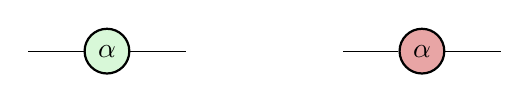
\begin{tikzpicture}
    \node [style=gn] (2) at (1,0) {\(\alpha\)};
    \node [style=rn] (1) at (5,0) {\(\alpha\)};
    \draw (0,0) to (2);
    \draw (2) to (2,0);
    \draw (4,0) to (1);
    \draw (1) to (6,0);
\end{tikzpicture}

Lahko imata poljubno število vhodov ali izhodov. V temu članku bomo pisali vhode na levi strani, izhode pa na desni strani pajka (izkaže pa se, da to ni pomembno). Kot primer, Z pajek z tremi vhodi in dvema izhodoma je

\begin{center}
  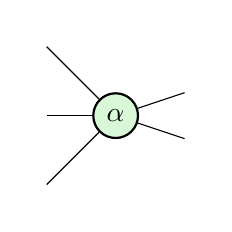
\begin{tikzpicture}
    \node (01) at (0, 0) {};
    \node (02) at (0, 1) {};
    \node (03) at (0, 2) {};
    \node [style=gn] (1) at (1.00, 1.00) {\(\alpha\)};
    \node (21) at (2, 0.66666) {};
    \node (22) at (2, 1.33333) {};
    \draw (01) to (1);
    \draw (02) to (1);
    \draw (03) to (1);
    \draw (1) to (21);
    \draw (1) to (22);
    %\end{pgfonlayer}
  \end{tikzpicture}.
\end{center}

Pajki ustrezajo linearnim preslikavam \cite[stran 39]{Backens}. Definiramo, da Z pajku z \(n\) vhodi in \(m\) izhodi pripada preslikava
\begin{align*}
    \ket{0}^{\otimes m} \bra{0}^{\otimes n} + e^{i\alpha}\ket{1}^{\otimes m} \bra{1}^{\otimes n}.
\end{align*}
Podobno definiramo X pajek z \(n\) vhodi in \(m\) izhodi kot
\begin{align*}
    \ket{+}^{\otimes m} \bra{+}^{\otimes n} + e^{i\alpha}\ket{-}^{\otimes m} \bra{-}^{\otimes n}.
\end{align*}

Iz teh pajkov si lahko definiramo nove konstrukcije. Tako lahko definiramo Hadamardova vrata kot
\begin{center}
    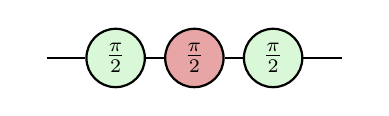
\begin{tikzpicture}
    \node (0) at (0.00, 0.00) {};
    \node [style=gn] (1) at (1, 0) {\(\frac\pi2\)};
    \node [style=rn] (2) at (2, 0) {\(\frac\pi2\)};
    \node [style=gn] (3) at (3, 0) {\(\frac\pi2\)};
    \node (4) at (4.00, 0.00) {};
    \draw (0) to (1);
    \draw (1) to (2);
    \draw (2) to (3);
    \draw (3) to (4);
    \end{tikzpicture}.
\end{center}
Ker jih bomo pogosto potrebovali, vpeljemo za ta vrata novo oznako
\begin{center}
    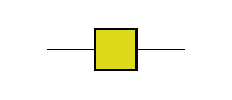
\begin{tikzpicture}
        \node (0) at (0, 0) {};
        \node [style=had] (h) at (1,0) {};
        \node (1) at (2,0) {};
        \draw (0) to (h);
        \draw (h) to (1);
    \end{tikzpicture}.
\end{center}
\subsection{Aksiomi}
\subsection{Primeri}
\subsection{Drobci}
\subsection{Kategorična slika}
\subsection{Dodatki}
\section{Kvantna mehanika z grafičnimi vezji}
\section{Poenostavjanje vezij}
\subsection{Quantomatic}
\section{Kvantni algoritmi in programiranje}
\subsection{Deutsch-Jozsov algoritem}
Najprej si definiramo nekaj pojmov.
\begin{definicija} Funkcija \(f:\{0,1\}^n\to \{0,1\}\) je konstantna, če \(\forall x\in\{0,1\}^n\sep f(x) = f(0,\ldots, 0)\).\end{definicija}
\begin{definicija}
    Funkcija \(f: \{0,1\}^n \to \{0,1\}\) je uravnotežena, če \(\exists S, U\subseteq \{0,1\}^n\) za katere \(\lvert S\rvert = \lvert U\rvert\) in \(f(S) = \{1\}, f(U) = \{0\}\)
\end{definicija}
Z drugimi besedami, funkcija je konstantna, če preslika vse argumente v isto vrednost in je uravnotežena, če preslika natanko polovico elementov v eno vrednost, drugo polovico pa v drugo.

Deutsch-Jozsov algoritemu podamo funkcijo \(f\) z zagotovilom, da je ali konstantna ali uravnotežena, ta nam pa v eni sami evaluaciji funkcije \(f\) odgovori katero izmed teh dveh opcij je.
\subsection{Kvantno iskanje}
Dano imamo funkcijo \(f: \{0,1\}^n\to \{0,1\}\) z zagotovilom, da se točno ena četrtina vhodov preslika v \(1\). Cilj je poiskati nek vhod \(x\in\{0,1\}^n\) pri katerem \(f(x) = 1\). S klasičnim algoritmom brez uporabe kvantne mehanike ugotovimo pravi odgovor z verjetnostjo \(0.25\), v najslabšem primeru pa moremo preveriti kar tri četrtine vhodov! Kvantni algoritm nam vedno da odgovor v eni evaluaciji funkcije.
\subsection{Računanje preko meritev}


\section*{Slovar strokovnih izrazov}

\geslo{Hilbert space}{Hilbertov prostor}
\geslo{observable}{opazljivka}
\geslo{state}{stanje}
\geslo{qubit}{kubit}
\geslo{balanced function}{uravnotežena funkcija}


\printbibliography
\end{document}

